\documentclass{beamer}
\usepackage{amssymb}
\usepackage{amsmath}
\usepackage{mathtools}
\usepackage{enumerate}
\usepackage{esint}
\usepackage{siunitx}
\usepackage{bbm}
\usepackage{graphicx}
\usepackage{caption}
\usepackage{subcaption}
\usepackage{wrapfig}
\usepackage{epstopdf}
\usepackage{float}
%\usepackage{cite}
\usepackage{tikz}
%\usepackage{collcell}
\usepackage{comment}
\usepackage{xcolor}
\usepackage[makeroom]{cancel}
\usepackage{nicefrac}
\usepackage{extarrows}

\newtheorem{thm}{Theorem}
\newtheorem{proposition}{Proposition}
\newtheorem{lem}{Lemma}
\newtheorem{cor}{Corollary}
\newtheorem{conjec}{Conjecture}
\newtheorem{remark}{Remark}

\usetikzlibrary{calc,arrows,quotes,angles}
%\usepackage{arydshln}
\usetikzlibrary{shapes,decorations}
\usepackage{multicol}
\usepackage{booktabs}
%\usepackage{beamerthemesplit}


\newcommand{\conj}[1]{\overline{#1}}
\newcommand{\newpar}{\vspace{5mm}\par}
\newcommand{\vnorm}[1]{\left\|#1\right\|}
\newcommand{\ket}[1]{\left\vert#1\right>}
\newcommand{\bra}[1]{\left<#1\right\vert}
\usepackage{amsthm}
\mode<presentation>{}

\newcommand{\light}[1]{\textcolor{gray}{#1}}
\newcommand{\hlight}[1]{\tikz[overlay, remember picture,baseline=-\the\dimexpr\fontdimen22\textfont2\relax]\node[rectangle,fill=blue!50,rounded corners,fill opacity = 0.2,draw,thick,text opacity =1] {$#1$};} 



\newcommand{\tabitem}{~~\llap{\textbullet}~~}

%%% Beamer colors
\usetheme{Madrid}
\usecolortheme{beaver}
\definecolor{Maroon}{cmyk}{0,0.8,0.68,0.32}
%\setbeamercolor*{palette primary}{fg=black,bg=Maroon}
%\setbeamercolor*{palette secondary}{fg=white,bg=structure.fg!60!white}
%\setbeamercolor*{palette tertiary}{fg=white,bg=structure.fg!90!white}
%\setbeamercolor*{palette quaternary}{fg=white,bg=black}

%\setbeamercolor*{sidebar}{use=structure,bg=structure.fg}

%\setbeamercolor*{palette sidebar primary}{fg=structure.fg!10}
%\setbeamercolor*{palette sidebar secondary}{fg=white}
%\setbeamercolor*{palette sidebar tertiary}{fg=structure.fg!50}
%\setbeamercolor*{palette sidebar quaternary}{fg=white}

%\setbeamercolor*{titlelike}{fg=structure.fg}

%\setbeamercolor*{separation line}{}
%\setbeamercolor*{fine separation line}{}

%\setbeamercolor{title}{fg=Maroon}
\setbeamercolor{block title}{fg=white, bg=red!75!black}
\setbeamercolor{block body}{bg=gray!30}
%\setbeamercolor{title}{use=structure, bg=gray!10}

\AtBeginSection[]
{
	\begin{frame}[noframenumbering]
	\frametitle{Outline}
	\tableofcontents[currentsection]
	\end{frame}
}


\begin{document}
\title{Cometric Association Schemes}
\date[March 11, 2019]{PhD Thesis Defense\\March 11, 2019}
\author{Brian Kodalen}
\institute[WPI]{Worcester Polytechnic Institute}
\frame{\titlepage}

\begin{frame}
\frametitle{Outline}
	\tableofcontents
\end{frame}

\section{Association schemes}
\begin{frame}
	\frametitle{Symmetric Association Scheme}
	A \textbf{symmetric association scheme} is an ordered pair $(X,\mathcal{R})$ where $X$ is a finite set and $\mathcal{R} = \left\{R_0,\dots,R_d\right\}$ is a partition of $X\times X$ into $d+1$ symmetric binary relations satisfying
	\begin{itemize}
		\item $R_0$ is the identity relation on $X$;
		\item for $0\leq i,j,k\leq d$, there exists $p^k_{ij}\in\mathbb{Z}$ such that
		\[\vert R_i(a)\cap R_j(b)\vert = p^k_{ij}\]
		whenever $(a,b)\in R_k$.
	\end{itemize}
\end{frame}

\begin{frame}
\frametitle{Example: Heawood Graph}
\centering
\scalebox{.95}{\begin{tikzpicture}[shorten >=1pt,auto,node distance=2cm,
thin,main node/.style = {circle,draw, minimum size = 5pt}]
\def\r{3.5}
\foreach \t in {0,...,13}
{{\node[main node] at ({\r*cos(180*(1+\t / 7))},{\r*sin(180*(\t / 7))}) (\t) {\t};}
{\node[main node] at ({\r*cos(180*(1+\t / 7))},{\r*sin(180*(\t / 7))}) (\t) {\t};}}
\draw[-] (13)--(0)--(1)--(2)--(3)--(4)--(5)--(6)--(7)--(8)--(9)--(10)--(11)--(12)--(13);
\draw[-] (0)--(5)--(4)--(9)--(8)--(13)--(12)--(3)--(2)--(7)--(6)--(11)--(10)--(1);
%base
\only<1->{
\foreach \t in {0}
{{\node[main node] at ({\r*cos(180*(1+\t / 7))},{\r*sin(180*(\t / 7))}) (\t) {\t};}
	{\node[main node,fill=blue] at ({\r*cos(180*(1+\t / 7))},{\r*sin(180*(\t / 7))}) (\t) {\t};}}
\node at (-5.5,3) () {};
\node at (5.5,3) () {};
\node at (-5.5,-3) () {};
\node at (5.5,-3) () {};
}
%dista2ce 1
\only<2->{
\foreach \t in {1,5,13}
{{\node[main node] at ({\r*cos(180*(1+\t / 7))},{\r*sin(180*(\t / 7))}) (\t) {\t};}
	{\node[main node,fill=red] at ({\r*cos(180*(1+\t / 7))},{\r*sin(180*(\t / 7))}) (\t) {\t};}}
\node at (-4,3) () {$p^1_{11} = 0$};}
%distance 2
\only<2->{
\foreach \t in {2,10,12,8,4,6}
{{\node[main node] at ({\r*cos(180*(1+\t / 7))},{\r*sin(180*(\t / 7))}) (\t) {\t};}
	{\node[main node,fill=green] at ({\r*cos(180*(1+\t / 7))},{\r*sin(180*(\t / 7))}) (\t) {\t};}}
\node at (4,3) () {$p^1_{12} = p^1_{21} = 2$};
}%\node at (-4,-3) () {$p^1_{21} = 2=p^1_{12}$};}
%distance 3
\only<2->{
\foreach \t in {3,7,9,11}
{{\node[main node] at ({\r*cos(180*(1+\t / 7))},{\r*sin(180*(\t / 7))}) (\t) {\t};}
	{\node[main node,fill=yellow] at ({\r*cos(180*(1+\t / 7))},{\r*sin(180*(\t / 7))}) (\t) {\t};}}
}%\node at (-4,-3) () {$p^3_{11} = 0$};}
\end{tikzpicture}}
\end{frame}

\begin{frame}
\frametitle{Relations need not be given by distance in a graph}

\[\begin{tikzpicture}[shorten >=1pt,auto,node distance=2cm,
thin,main node/.style = {circle,draw}]
\only<1>{\node[main node,fill=white] at (-.5,.5) (y1) {};
\node[main node,fill=white] at (-1.5,-.5) (y2) {};
\node[main node,fill=white] at (-2.5,-1.5) (y3) {};
\node[main node,fill=white] at (-3.5,-2.5) (y4) {};
\node[main node,fill=white] at (2.5,0.5) (r1) {};
\node[main node,fill=white] at (3.5,-.5) (r2) {};
\node[main node,fill=white] at (4.5,-1.5) (r3) {};
\node[main node,fill=white] at (5.5,-2.5) (r4) {};
\node[main node,fill=white] at (-1.6,-5) (b1) {};
\node[main node,fill=white] at (.2,-5) (b2) {};
\node[main node,fill=white] at (1.8,-5) (b3) {};
\node[main node,fill=white] at (3.6,-5) (b4) {};}
\only<2>{\node[main node,fill=blue] at (-.5,.5) (y1) {};
	\node[main node,fill=white] at (-1.5,-.5) (y2) {};
	\node[main node,fill=white] at (-2.5,-1.5) (y3) {};
	\node[main node,fill=white] at (-3.5,-2.5) (y4) {};
	\node[main node,fill=white] at (2.5,0.5) (r1) {};
	\node[main node,fill=white] at (3.5,-.5) (r2) {};
	\node[main node,fill=white] at (4.5,-1.5) (r3) {};
	\node[main node,fill=white] at (5.5,-2.5) (r4) {};
	\node[main node,fill=white] at (-1.6,-5) (b1) {};
	\node[main node,fill=white] at (.2,-5) (b2) {};
	\node[main node,fill=white] at (1.8,-5) (b3) {};
	\node[main node,fill=white] at (3.6,-5) (b4) {};}
\only<3->{\node[main node,fill=blue] at (-.5,.5) (y1) {};
	\node[main node,fill=green] at (-1.5,-.5) (y2) {};
	\node[main node,fill=green] at (-2.5,-1.5) (y3) {};
	\node[main node,fill=green] at (-3.5,-2.5) (y4) {};
	\node[main node,fill=yellow] at (2.5,0.5) (r1) {};
	\node[main node,fill=red] at (3.5,-.5) (r2) {};
	\node[main node,fill=red] at (4.5,-1.5) (r3) {};
	\node[main node,fill=red] at (5.5,-2.5) (r4) {};
	\node[main node,fill=yellow] at (-1.6,-5) (b1) {};
	\node[main node,fill=red] at (.2,-5) (b2) {};
	\node[main node,fill=red] at (1.8,-5) (b3) {};
	\node[main node,fill=red] at (3.6,-5) (b4) {};}

	\only<1-3>{\draw[-] (y1)-- (r2);
	\draw[-] (y1)-- (r3);
	\draw[-] (y1)-- (r4);
	\draw[-] (y2)-- (r1);
	\draw[-] (y2)-- (r3);
	\draw[-] (y2)-- (r4);
	\draw[-] (y3)-- (r2);
	\draw[-] (y3)-- (r1);
	\draw[-] (y3)-- (r4);
	\draw[-] (y4)-- (r2);
	\draw[-] (y4)-- (r3);
	\draw[-] (y4)-- (r1);
	\draw[-] (b1)-- (r2);
	\draw[-] (b1)-- (r3);
	\draw[-] (b1)-- (r4);
	\draw[-] (b2)-- (r1);
	\draw[-] (b2)-- (r3);
	\draw[-] (b2)-- (r4);
	\draw[-] (b3)-- (r2);
	\draw[-] (b3)-- (r1);
	\draw[-] (b3)-- (r4);
	\draw[-] (b4)-- (r2);
	\draw[-] (b4)-- (r3);
	\draw[-] (b4)-- (r1);
	\draw[-] (y1)-- (b2);
	\draw[-] (y1)-- (b3);
	\draw[-] (y1)-- (b4);
	\draw[-] (y2)-- (b1);
	\draw[-] (y2)-- (b3);
	\draw[-] (y2)-- (b4);
	\draw[-] (y3)-- (b2);
	\draw[-] (y3)-- (b1);
	\draw[-] (y3)-- (b4);
	\draw[-] (y4)-- (b2);
	\draw[-] (y4)-- (b3);
	\draw[-] (y4)-- (b1);}
	
	\only<4>{\draw[-,very thin,gray] (y1)-- (r2);
		\draw[-,very thin,gray] (y1)-- (r3);
		\draw[-,very thin,gray] (y1)-- (r4);
		\draw[-,very thin,gray] (y2)-- (r1);
		\draw[-,very thin,gray] (y2)-- (r3);
		\draw[-,very thin,gray] (y2)-- (r4);
		\draw[-,very thin,gray] (y3)-- (r2);
		\draw[-,very thin,gray] (y3)-- (r1);
		\draw[-,very thin,gray] (y3)-- (r4);
		\draw[-,very thin,gray] (y4)-- (r2);
		\draw[-,very thin,gray] (y4)-- (r3);
		\draw[-,very thin,gray] (y4)-- (r1);
		\draw[-,very thin,gray] (b1)-- (r2);
		\draw[-,very thin,gray] (b1)-- (r3);
		\draw[-,very thin,gray] (b1)-- (r4);
		\draw[-,very thin,gray] (b2)-- (r1);
		\draw[-,very thin,gray] (b2)-- (r3);
		\draw[-,very thin,gray] (b2)-- (r4);
		\draw[-,very thin,gray] (b3)-- (r2);
		\draw[-,very thin,gray] (b3)-- (r1);
		\draw[-,very thin,gray] (b3)-- (r4);
		\draw[-,very thin,gray] (b4)-- (r2);
		\draw[-,very thin,gray] (b4)-- (r3);
		\draw[-,very thin,gray] (b4)-- (r1);
		\draw[-,very thin,gray] (y1)-- (b2);
		\draw[-,very thin,gray] (y1)-- (b3);
		\draw[-,very thin,gray] (y1)-- (b4);
		\draw[-,very thin,gray] (y2)-- (b1);
		\draw[-,very thin,gray] (y2)-- (b3);
		\draw[-,very thin,gray] (y2)-- (b4);
		\draw[-,very thin,gray] (y3)-- (b2);
		\draw[-,very thin,gray] (y3)-- (b1);
		\draw[-,very thin,gray] (y3)-- (b4);
		\draw[-,very thin,gray] (y4)-- (b2);
		\draw[-,very thin,gray] (y4)-- (b3);
		\draw[-,very thin,gray] (y4)-- (b1);}
	\only<4>{\draw[-,yellow,thick] (y1) --(b2) -- (r1);
	\draw[-,green,thick] (y1) -- (b3) -- (y2);}
\end{tikzpicture}\]
\end{frame}

\begin{comment}
\begin{frame}
\frametitle{$P$-polynomial (metric)}
$(X,\mathcal{R})$ is {\em$P$-polynomial} if we can order the relations so that:
\[p^k_{ij}\begin{cases}
= 0, & k>i+j \text{ or } k<\vert i-j\vert\\
> 0, & k = i+j
\end{cases}\]\pause
Examples:
\begin{multicols}{2}
	\begin{itemize}
		\item SRGs
		\item Generalized Quadrangles
		\item Projective Planes
		\item Moore Graphs
	\end{itemize}
\end{multicols}
\end{frame}
\end{comment}

\begin{frame}
\frametitle{Bose-Mesner Algebra}
Let $A_i$ denote the adjacency matrix of the graph $(X,R_i)$.
\[\mathbb{A} = \text{span}_\mathbb{R}(A_0,A_1,\dots,A_d)\]
\[A_iA_j = \sum_k p^k_{ij}A_k\]\pause


\only<1-2,4->{\[\underset{(symmetric)}{A_i = A_i^T}\implies p^k_{ij} = p^k_{ji}\implies \underset{(commutative)}{A_iA_j = A_jA_i}\]}\pause
\only<3>{
\[\xcancel{\light{\underset{(symmetric)}{A_i = A_i^T}}}\light{\implies} p^k_{ij} = p^k_{ji}\implies \underset{(commutative)}{A_iA_j = A_jA_i}\]}\pause\pause

\vfill
Second basis using projection matrices (idempotents):
\[\mathbb{A} = \text{span}_\mathbb{R}(E_0,E_1,\dots,E_d)\]

\end{frame}


\begin{frame}
\frametitle{Q-polynomial (cometric)}
\[A_i\circ A_j = \delta_{ij}A_i\implies \mathbb{A}\text{ is closed under }\circ\]\pause\vfill
There exists ``Krein parameters" $q^k_{ij}$ such that:
\[E_i\circ E_j = \frac{1}{\vert X\vert}\sum_{k} q^k_{ij}E_k\]\pause
$(X,\mathcal{R})$ is {\em $Q$-polynomial} if we can order the idempotents so that:
\[q^{k}_{ij}\begin{cases}
=0 & k>i+j\text{ or }k<\vert i-j\vert\\
>0 & k = i+j\\
\end{cases}\]

%\begin{itemize}
%\item\textit{Q-antipodal} if $q^{k}_{dd}>0 \implies k\in\left\{0,d\right\}$\\
%\item\textit{Q-bipartite} if $q^{k}_{ij}=0 \text{ whenever } i+j+k\text{ is odd.}$
%\end{itemize}
\end{frame}

\begin{frame}
	\frametitle{$P$-polynomial vs. $Q$-polynomial}
$P$-polynomial (metric):
\[p^{k}_{ij}\begin{cases}
=0 & k>i+j\text{ or }k<\vert i-j\vert\\
>0 & k = i+j\\
\end{cases}\]
\begin{itemize}
	\item $R_i$ given by distance $i$ in a ``distance-regular graph"
	\item extensively studied for decades
\end{itemize}\vfill
$Q$-polynomial (cometric):
\begin{itemize}
	\item no known combinatorial defining property
	\item studied more within the last 20 years
\end{itemize}


\end{frame}

\begin{comment}
\begin{frame}
	\frametitle{$P$-polynomial vs. $Q$-polynomial}
	\begin{table}
		\centering
		\begin{tabular}{lll}
			\multicolumn{3}{c}{} \\%[.5\normalbaselineskip]
			Theorem & Metric & Cometric \\
			\midrule
			1.~Multiple polynomial orderings& {\footnotesize1980} & {\footnotesize1998-2014} \\
			 &  & (Suzuki) \\[.5\normalbaselineskip]\pause
			2.~Systems of Imprimitivity & {\footnotesize 1971-1980} & {\footnotesize 1998-2010} \\
			 &  & (Suzuki) \\[.5\normalbaselineskip]\pause
			3.~Unimodality of parameters & {\footnotesize1978} & {\footnotesize still open} \\[.5\normalbaselineskip]
			\midrule
		\end{tabular}
	\end{table}
\end{frame}
\end{comment}

\begin{frame}
	\frametitle{A conjecture of Bannai \& Ito}
	\begin{conjec}[Bannai and Ito]
		For $d$ sufficiently large, a primitive association scheme with $d$ classes is metric if and only if it is cometric.
	\end{conjec}\pause
	\vspace{1cm}
	\[\text{How about low $d$?}\]\pause
	\[\text{We will consider }d\in\left\{3,4\right\}\]
\end{frame}

\begin{comment}
\begin{frame}
	\frametitle{$Q$-polynomial association schemes with low class number}
	\begin{tikzpicture}
		\def\s{2}
		\def\x{0}
		\def\y{0}
		\def\t{2}
		\def\l{.2}
		\def\b{7.5}
		\def\labeloffset{1.5}
		\node at (\x-2.5,\y) (classes) {d};
		\draw[-] (\x-3,\y-\l) -- (\x-2,\y-\l) -- (\x-2,\y);
		
		\draw[-] (\x-3,\y-\t/2) -- (\x-2,\y-\t/2);
		\node at (\x-2.5,\y-\t) () {3};
		\draw[-] (\x-3,\y-3*\t/2) -- (\x-2,\y-3*\t/2);
		\node at (\x-2.5,\y-2*\t) () {4};
		\draw[-] (\x-3,\y-5*\t/2) -- (\x-2,\y-5*\t/2);
		\node at (\x-2.5,\y-3*\t) () {5};
		\draw[-] (\x-3,\y-7*\t/2) -- (\x-2,\y-7*\t/2);
		
		\only<2>{\draw[-,color=blue] (\x-3,\y-\t/2) -- (\x-2,\y-\t/2);
		\node[color=blue] at (\x-2.5,\y-\t) () {3};
		\draw[-,color=blue] (\x-2,\y-\t/2) -- (\x,\y);
		\draw[-,color=blue] (\x-2,\y-3*\t/2) -- (\x,\y-\b);}
		
		\only<2-3>{\draw[-,color=blue] (\x-3,\y-3*\t/2) -- (\x-2,\y-3*\t/2);}
		
		\only<3>{\node[blue] at (\x-2.5,\y-2*\t) () {4};
		\draw[-,color=blue] (\x-2,\y-3*\t/2) -- (\x,\y);
		\draw[-,color=blue] (\x-2,\y-5*\t/2) -- (\x,\y-\b);}
		
		\only<3-4>{\draw[-,blue] (\x-3,\y-5*\t/2) -- (\x-2,\y-5*\t/2);}
		
		\only<4>{\node[blue] at (\x-2.5,\y-3*\t) () {5};
		\draw[-,blue] (\x-3,\y-7*\t/2) -- (\x-2,\y-7*\t/2);
		\draw[-,color=blue] (\x-2,\y-5*\t/2) -- (\x,\y);
		\draw[-,color=blue] (\x-2,\y-7*\t/2) -- (\x,\y-\b);}
		
		
		
		\draw[-] (\x+2*\s,\y) -- (\x+2*\s,\y-\b);
		\draw[-] (\x,\y-2*\s) -- (\x+4*\s,\y-2*\s);
		\node at (\x+\s,\y-\s+\labeloffset) (prim) {primitive};
		\node at (\x+3*\s,\y-\s+\labeloffset) (bip) {$Q$-bipartite};
		\node at (\x+\s,\y-3*\s+\labeloffset) (ant) {$Q$-antipodal};
		\node at (\x+3*\s,\y-3*\s+\labeloffset) (both) {both};
		\only<1>{
			\node[align=center] at (\x+\s,\y-\s) (prim) {Spherical \\ $d$-distance set};
			\node[align=center] at (\x+3*\s,\y-1.2*\s) (bip) {Inner products: \\ $\left\{-1,\pm \alpha,\dots\right\}$\\\\``lines through\\ the origin"};
			\node[align=center] at (\x+\s,\y-3*\s) (ant) {Fibers with \\ inner products:\\ $1>\beta_1>\alpha_2>\beta_2>\dots$};
			\node[align=center] at (\x+3*\s,\y-3*\s) (both) {};
		}
		\only<2>{
				\node[align=center] at (\x+\s,\y-\s) (prim) {Spherical\\$3$-distance set};
				\node[align=center] at (\x+3*\s,\y-\s) (bip) {Equiangular lines \\ (two-graphs)\\\\(Haantjes `48)};
				\node[align=center] at (\x+\s,\y-3*\s) (ant) {``\textit{LSSD}"\\$[iff]$\\(Cameron `72)};
				\node[align=center] at (\x+3*\s,\y-3*\s) (both) {Trivial $LSSD$\\$[iff]$\\ uses $(v,1,0;2)$};
		}
		\only<3>{
			\node[align=center] at (\x+\s,\y-\s) (prim) {Spherical\\$4$-distance set};
			\node[align=center] at (\x+3*\s,\y-\s) (bip) {Two angles\\ (w/ $90^\circ$)\\\\Double covers of SRGs};
			\node[align=center] at (\x+\s,\y-3*\s) (ant) {``\textit{LSSRD}"\\$[iff]$\\(Higman `95)};
			\node[align=center] at (\x+3*\s,\y-3*\s) (both) {Mutually Unbiased \\ Bases\\$[iff]$\\(DGS `75)};
		}
		\only<4>{
			\node[align=center] at (\x+\s,\y-\s) (prim) {Spherical\\$5$-distance set};
			\node[align=center] at (\x+3*\s,\y-\s) (bip) {Two angles\\ (neither $90^\circ$)\\\\Double covers of SRGs};
			\node[align=center] at (\x+\s,\y-3*\s) (ant) {``\textit{LSSRD}"\\$[iff]$\\(Higman `95)};
			\node[align=center] at (\x+3*\s,\y-3*\s) (both) {bip-double of\\ SRG $\left(q_{11}^1=0\right)$\\$[iff]$};
		}
	\end{tikzpicture}
\end{frame}
\end{comment}

\section{Realizability vs feasibility}

\begin{frame}
	\frametitle{Parameter Constraints}
	\[A_i = \sum_j P_{ji}E_j,\qquad E_j=\frac{1}{\vert X\vert}\sum_i Q_{ij}A_i.\]\pause
	\begin{figure}[h]
	\includegraphics[scale=.3]{Feas1.PNG}
	\end{figure}\pause
	\[p^k_{0j} = \delta_{kj},\qquad\onslide<4>{\sum_{\ell}q^\ell_{ij}q^m_{\ell h} = \sum_{\ell}q^m_{i\ell}q^\ell_{jh}.} \]
\end{frame}

\begin{frame}
	\frametitle{Parameter Constraints}
	\vspace{-.5cm}\[
	\begin{tikzpicture}
	\node at (0,0) (pic) {\includegraphics[scale=.45,trim={0cm 0cm 0cm 0cm}, clip]{Feas2.PNG}};
	\only<2>{\draw[red,ultra thick, rounded corners] (-4,3.3) rectangle (-2.7,2.8);}
	\only<2>{\draw[red,ultra thick, rounded corners] (0,.2) rectangle (2.7,.8);}
	\end{tikzpicture}\]
\end{frame}

\begin{frame}
	\frametitle{Feasibility}
	A \emph{parameter set} consists of
	\begin{itemize}
		\item all intersection numbers $p^k_{ij}$;
		\item all Krein parameters $q^k_{ij}$;
		\item both eigenmatrices $P$ and $Q$.
	\end{itemize}\vfill\pause

	A parameter set is \emph{feasible} if
	\begin{itemize}
		\item each $p^k_{ij}$ is integral (and non-negative);
		\item each $q^k_{ij}$ is non-negative;
		\item all properties on the previous slide are fulfilled;
		\item the multiplicities $m_j:=q^0_{jj}$ satisfy the absolute bound.
	\end{itemize}\pause\vfill
A parameter set is \emph{realizable} if there exists a scheme with those parameters.
\end{frame}
\begin{frame}
\frametitle{Realizability vs. Feasibility}\vspace{-.5cm}
\only<1>{\[\includegraphics[scale=.4,trim={0cm 0cm 22.3cm 0cm},clip]{prim1.PNG}\]}
\only<2>{\[\includegraphics[scale=.4,trim={0cm 3.35cm 22.3cm 0cm},clip]{prim2.PNG}\]}
\\
Image clipped from Williford's tables: \underline{http://www.uwyo.edu/jwilliford/files/data/qprim3table.html}
\end{frame}

\begin{frame}
	\frametitle{Isomorphic algebras}
	Let $L_i^* = \left[q^k_{ij}\right]_{k,j}$.\\\pause
	Since $\sum_{\ell}q^\ell_{ij}q^m_{\ell h} = \sum_{\ell}q^m_{i\ell}q^\ell_{jh}$, we find
	\[L_i^*L_j^* =\sum_k q^k_{ij}L_{k}^*.\qquad\onslide<3->{\left(\text{ Recall: }E_i\circ E_j =\frac{1}{\vert X\vert}\sum_k q^k_{ij}E_{k}\right)}\]\pause\pause
	Then $\phi^*:\mathbb{A}\rightarrow \left<L_0^*,\dots,L_d^*\right>$ via
	\[\phi^*\left(E_i\right) = \frac{1}{\vert X\vert}L_i^*\]
	is an algebra isomorphism mapping entrywise products to matrix products.
\end{frame}

\begin{frame}
\frametitle{Sch\"{o}nberg's Theorem}
A function $f:[-1,1]\rightarrow \mathbb{R}$ is \textit{positive definite} if, for every finite subset $X$, $f\circ\left(G_X\right)\succeq 0$, where $G_X$ is the Gram matrix of $X$.\vspace{1cm}
\begin{thm}[Sch\"{o}nberg,`45]
	A continuous function $f:[-1,1]\rightarrow \mathbb{R}$ is positive definite if and only if $f$ is expressible as a non-negative linear combination of the Gegenbauer polynomials.
\end{thm}

\end{frame}

\begin{frame}
\frametitle{Gegenbauer Polynomials}
\[\begin{aligned}
Q_0^{(m)} &= 1 \qquad Q_1^{(m)} = t\\
Q_{k}^{(m)} &= \frac{(2k+m-4)tQ_{k-1}^{(m)}(t)-(k-1)Q_{k-2}^{(m)}(t)}{k+m-3}
\end{aligned}\]\vfill\pause
$$Q_0^{(m)}(t)=1\qquad	Q_1^{(m)}(t)=t\qquad Q_2^{(m)}(t)=\frac{mt^2 - 1}{m-1}$$
\begin{center}
\scalebox{.9}{$Q_3^{(m)}(t)=\frac{(m+2)t^3 - 3t}{m-1}\qquad Q_4^{(m)}(t)=\frac{(m+4)(m+2)t^4 - 6(m+2)t^2+3}{m^2-1}$}\\\vspace{4mm}
\scalebox{.9}{$Q_5^{(m)}(t)=\frac{(m+6)(m+4)t^5-10(m+4)t^3+15t}{m^2-1}$}%\\\vspace{2mm}
%\scalebox{.9}{$Q_6^m(t)=\frac{(m+8)(m+6)(m+4)t^6-15(m+6)(m+4)t^4+45(m+4)t^2-15}{(m+3)(m+1)(m-1)}$}
\end{center}
\end{frame}

\begin{frame}
	\begin{theorem}[K.]
		Let $(X,\mathcal{R})$ be an association scheme with minimal idempotents $E_0,\dots,E_d$ and matrices of Krein parameters $\displaystyle{L_0^*,\dots,L_d^*}$. Fix some $E_i$, $0\leq i\leq d$, and let $m_i:=\text{rank}\left(E_i\right)$. Then for any choice of $\ell>0$, there exist non-negative constants $\theta_{\ell j}$, $0\leq j\leq d$, such that
		\begin{equation*}
		Q_\ell^{m_i}\circ\left(\frac{\vert X\vert}{m_i}E_i\right) = \sum_j \theta_{\ell j} E_j;\qquad	Q_\ell^{m_i}\left(\frac{1}{m_i}L_i^*\right) = \frac{1}{\vert X\vert}\sum_j \theta_{\ell j} L_j^*.
		\end{equation*}
	\end{theorem}\pause
	\begin{corollary}[K.]
		If a parameter set $\left\{q_{ij}^k\right\}$ is realizable then, for all $\ell\geq 0$ and all $0\leq i\leq d$, \[Q^{m_i}_\ell\left(\frac{1}{m_i}L_i^*\right)\geq 0.\]
	\end{corollary}
\end{frame}

\begin{comment}
\begin{frame}
\frametitle{$Q$-polynomial implications}
\begin{theorem}[K.]
	Suppose we have a feasible parameter set for a cometric association scheme with Krein array $\iota^*(X,\mathcal{R}) = \left\{m,b^*_1,\dots,b^*_{d-1};1,c_2^*\dots,c^*_{d}\right\}$ where $m>2$. Define $b_{j-1}^* = c_j^*=a_j^*=0$ for $j>d$. Then the scheme is realizable only if
	\begin{itemize}
		\item $\left(a_1^*\right)^2 + b_1^*c_2^* \geq\frac{2m(m-1)}{m+2},$
		\item $\left(a_1^*\right)^2+2a_1^*a_2^*+c_2^*q^2_{22}\geq \frac{4m(m-2)}{m+4},$
		\item $\frac{6m(m-1)(m-4)}{(m+4)(m+6)}+\frac{\left(3a_1^*\left(a_1^*+a_2^*\right)+c_2^*q_{22}^2\right)b_1^*c_2^*+\left(a_1^*\right)^4}{m}\geq \frac{(7m-18)\left(\left(a_1^*\right)^2+b_1^*c_2^*\right)}{m+6},$
		\item $\sum_{i=1}^3\left(b_i^*c_{i+1}^* + a_i^*\sum_{j=i}^3 a_j^*\right)\leq \frac{3(3m-2)}{m+6}.$
		\item $\frac{16m(m-1)}{(m+4)(m+8)} + \frac{\left(a_1^*\right)^4 + \left(3a_1^*\left(a_1^*+a_2^*\right)+c_2^*q_{22}^2\right)b_1^*c_2^*}{(m-2)m}\geq \frac{12\left(\left(a_1^*\right)^2+b_1^*c_2^*\right)}{m+8},$
	\end{itemize}
	Additionally, if $a_1^*>0$, then
	\begin{itemize}
		\item $\left(a_1^*\right)^2 + b_1^*c_2^*\left(2 + \frac{a_2^*}{a_1^*}\right)\geq \frac{4m(2m-3)}{m+6},$
		\item $\left(a_1^*\right)^2+2a_1^*a_2^*-\left(a_2^*\right)^2+2c_2^*q_{22}^2+\frac{b_2^*c_3^*\left(a_3^*-a_1^*\right)-ma_2^*}{a_1^*+a_2^*}\geq\frac{6m(m-4)}{m+6}.$
	\end{itemize}
\end{theorem}
\end{frame}
\end{comment}

\begin{frame}
\frametitle{$Q$-polynomial Consequences}
\begin{thm}[K.]
Let $(X,\mathcal{R})$ be a $Q$-polynomial association scheme with $m=\text{rank}\left(E_1\right)$. Then,
\begin{itemize}
\item $\left(q_{11}^1\right)^2 + q_{12}^1q_{11}^2\geq\frac{2m(m-1)}{m+2}$
\item $\left(q_{11}^1\right)^2 + \left(2+\frac{q^2_{12}}{q^1_{11}}\right)q_{12}^1q_{11}^2\geq\frac{4m(2m-3)}{m+6}$
\end{itemize}
\end{thm}
Proof technique: Apply $Q_4^{(m)}(t)$ and $Q_5^{(m)}(t)$ to $\frac{\vert X\vert}{m}E_1$.
\vfill\vfill
{\tiny Rules out, e.g.:
\[\begin{aligned}\left\{(441; 20)\right.&; (576; 23); (729; 26); (1015; 28); (1240; 30); (1548; 35);\\ &\left. (1836; 35); (1944; 29); (1976; 25); (1000; 27); (1331; 30)\right\}
\end{aligned}\]}
\end{frame}

\begin{frame}
\frametitle{Example}
\[P = \left[\begin{array}{rrrr}
1 & 100 & 240 & 100\\
1 & 37 & -12 & -26\\
1 & 2 & -12 & 9\\
1 & -5 & 9 & -5
\end{array}\right],\qquad Q = \left[\begin{array}{rrrr}
1 & 20 & 180 & 240\\
1 & \nicefrac{37}{5} & \nicefrac{18}{5} & -12\\
1 & -1 & -9 & 9\\
1 & \nicefrac{-26}{5} & \nicefrac{91}{5} & -12
\end{array}\right].\]\pause
Applying $G^{(20)}_0,\dots,G^{(20)}_6$ to $L_1^*$ and recording each first column gives:
\only<1-2>{\[\begin{bmatrix}%{cccccrc}
441 & 0 & 0 & 4.95 & 0.43 & -0.11 & 0.93 \\
0 & 22.05 & 4.5 & 0.38 & 0.67 & 0.84 & 0.97 \\
0 & 0 & 1.95 & 1.09 & 0.81 & 1 & 1.04 \\
0 & 0 & 0 & 0.97 & 1.17 & 1.02 & 0.98 
\end{bmatrix}.\]}\pause
\only<3>{\[\begin{bmatrix}%{cccccrc}
	441 & 0 & 0 & 4.95 & 0.43 & \hlight{-0.11} & 0.93 \\
	0 & 22.05 & 4.5 & 0.38 & 0.67 & 0.84 & 0.97 \\
	0 & 0 & 1.95 & 1.09 & 0.81 & 1 & 1.04 \\
	0 & 0 & 0 & 0.97 & 1.17 & 1.02 & 0.98 
	\end{bmatrix}.\]}
This parameter set is not realizable!
\end{frame}



\begin{comment}
\begin{frame}
	\frametitle{Background}
	\begin{itemize}
		\item[] Brouwer \& Mesner, 1985
		\item The vertex connectivity of a SRG is equal to its valency, and the only disconnecting sets of minimum size are the neighborhoods of its vertices.
	\end{itemize}
\only<1>{\begin{minipage}{.5495\textwidth}
		\vfill\hfill
\end{minipage}}
\only<2->{\begin{minipage}{.56\textwidth}
	\begin{itemize}
		\item[] Brouwer \& Koolen, 2009
		\item Replaced ``SRG" with ``DRG".
	\end{itemize}\hfill
\end{minipage}}
\begin{minipage}{.4\textwidth}
	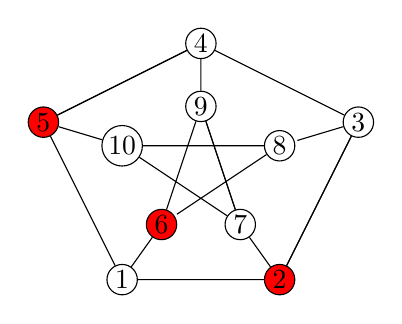
\begin{tikzpicture}[shorten >=1pt,auto,node distance=2cm,
	thin,main node/.style = {circle,draw, inner sep = 1pt, minimum size = 3pt}]
	\node[main node] at (0,0) (1) {1};
	\node[main node,fill=red] at (.5,.7) (2) {6};
	\node[main node] at (1.5,.7) (3) {7};
	\node[main node] at (1,2.2) (4) {9};
	\node[main node,fill=red] at (2,0) (5) {2};
	\node[main node] at (2,1.7) (6) {8};
	\node[main node] at (0,1.7) (7) {10};
	\node[main node,fill=red] at (-1,2) (8) {5};
	\node[main node] at (3,2) (9) {3};
	\node[main node] at (1,3) (10) {4};
	\draw[-] (1)--(5)--(9)--(10)-- (8)--(1)--(2)--(4)--(3)--(7)--(6)--(2);
	\draw[-] (7)--(8)--(10)--(4)--(3)--(5)--(9)--(6);
	\end{tikzpicture}
	\end{minipage}
\end{frame}

\begin{frame}
\frametitle{Theorem on Connectivity}
\begin{thm}[K.,Martin]
	Let $(X,\mathcal{R})$ be a symmetric association scheme. Assume the graph $\Gamma = (X,R_i)$ is connected and not complete multipartite. Let $H=H_i$ be the corresponding unweighted distribution diagram on $\left\{0,1,\dots,d\right\}$. The following are equivalent:
	\begin{enumerate}
		\item there exists $a\in X$ for which the subgraph $\Gamma\backslash a^\perp$ is connected;
		\item for all $a\in X$, the subgraph $\Gamma\backslash a^\perp$ is connected;
		\item the subgraph $H\backslash \left\{0,i\right\}$ is connected;
		\item $\Gamma$ contains no twins.
	\end{enumerate}
\end{thm}
\[H_i = \Gamma(\left\{0,\dots,d\right\},E_i)\qquad E_i = \left\{(k,j):p^k_{ij} >0\right\}\]
\end{frame}


\begin{frame}
\frametitle{$\Gamma \rightarrow H$ via the projection map }
\[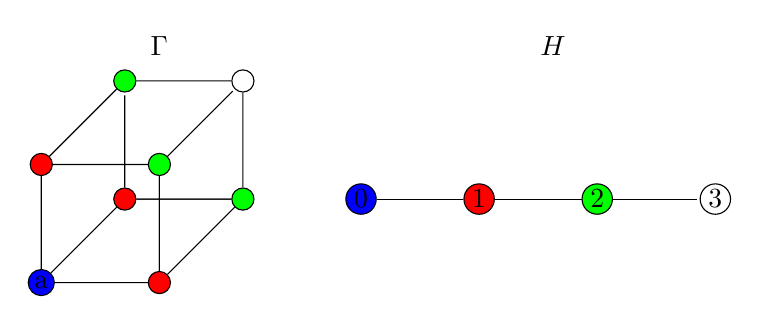
\begin{tikzpicture}[shorten >=1pt,auto,node distance=1.5cm,
thin,main node/.style = {circle,draw, inner sep = 1pt, minimum size = 8pt}]
\node at (1.5,3) (g) {$\Gamma$};
\node at (6.5,3) (h) {$H$};
\node[main node,fill=blue] (1) {a};
\node[main node,fill=red] [right of = 1](2) {};
\node[main node,fill=red] [above of = 1](3) {};
\node[main node,fill=green] [right of = 3](4) {};
\node[main node,fill=red] [above right of = 1](5) {};
\node[main node,fill=green] [right of = 5](6) {};
\node[main node,fill=green] [above of = 5] (7) {};
\node[main node] [right of = 7](8) {};

\node[main node,fill=blue] [right of = 6](9) {0};
\node[main node,fill=red] [right of = 9](10) {1};
\node[main node,fill=green] [right of = 10](11) {2};
\node[main node] [right of = 11](12) {3};

\draw[-] (3)--(1)--(2)--(4)--(3)--(7)--(8)--(6)--(5)--(7);
\draw[-] (1)--(5)--(6)--(2)--(4)--(8);
\draw[-] (9)--(10)--(11)--(12);


%\only<3->{\draw[->,green,line width = 0.5mm] (7) -- (8);
% \draw[->,green,line width = 0.5mm] (8) -- (4);
% \draw[->,green,line width = 0.5mm] (11) -- (12);
%\draw[->,green,line width = 0.5mm] (12) -- (11);}
%\only<2->{\draw[->,purple,line width = 0.5mm] (1)->(2);
%\draw[->,purple,line width = 0.5mm] (2)->(4);
%\draw[->,purple,line width = 0.5mm] (4)->(3);
%\draw[->,purple,line width = 0.5mm] (9)->(10);
%\draw[->,purple,line width = 0.5mm] (10)->(11);
%\draw[->,purple,line width = 0.5mm] (11)->(10);}
\end{tikzpicture}\]
\begin{itemize}
	\item Need to show $\Gamma\backslash a^\perp$ is connected if and only if $H\backslash \left\{0,1\right\}$ is as well.
\end{itemize}
\end{frame}

\begin{frame}
	\frametitle{$\Gamma_1$ and $H_1$ for the group $S_4$}
	\[\begin{tikzpicture}[shorten >=1pt,auto,node distance=1.5cm,
	thin,main node/.style = {draw, circle, inner sep = 1pt, minimum size = 8pt}]
	\node at (0,3.5) (g) {$\Gamma$};
	\node at (6,3) (h) {$H$};
	\def\r{2};
	\def\R{3};
	\foreach\t in {0,...,11}{
	\foreach\s in {2,3}{
	\node[main node] at ({\s*cos(30*\t)},{\s*sin(30*\t)}) (\t\s) {};
	}}
	
	
	

	\node[main node,fill=blue] at (93) {};
	
	\node[main node,fill=red] at (103) {};
	\node[main node,fill=red] at (83) {};
	\node[main node,fill=red] at (92) {};
	\node[main node,fill=red] at (72) {};
	\node[main node,fill=red] at (112) {};
	\node[main node,fill=red] at (32) {};
	
	\node[main node,fill=green] at (62) {};
	\node[main node,fill=green] at (02) {};
	\node[main node,fill=green] at (33) {};
	
	\node[main node,fill=yellow] at (63) {};
	\node[main node,fill=yellow] at (43) {};
	\node[main node,fill=yellow] at (23) {};
	\node[main node,fill=yellow] at (03) {};
	\node[main node,fill=yellow] at (52) {};
	\node[main node,fill=yellow] at (12) {};
	
	\node[main node,fill=black] at (13) {};
	\node[main node,fill=black] at (53) {};
	\node[main node,fill=black] at (73) {};
	\node[main node,fill=black] at (113) {};
	\node[main node,fill=black] at (42) {};
	\node[main node,fill=black] at (22) {};
	\node[main node,fill=black] at (82) {};
	\node[main node,fill=black] at (102) {};
	
	\node[main node,fill=blue] at (6,-1) (b) {};
	\node[main node,fill=red] at (6,0) (r) {};
	\node[main node,fill=green] at (5,1) (g) {};
	\node[main node,fill=black] at (7,1) (bl) {};
	\node[main node,fill=yellow] at (6,2) (y) {};
	
	\only<1>{\foreach\t in {0,...,11}{
				\draw let \n1={int(mod(\t+1,12))} in (\t3) -- (\n13);
				\draw let \n1={int(mod(\t+7,12))} in (\t2) -- (\n12);
			\draw (\t\r) -- (\t\R);
			\draw let \n2={int(mod(\t+2,12))} in (\t\r) to [bend right=15] (\n2\R);
			\draw let \n3={int(mod(\t+2,12))} in (\t\R) to [bend right=15] (\n3\r);
			\draw let \n4={int(mod(\t+6,12))} in (\t\R) to [bend left=15] (\n4\r);}
		\draw[-] (b) -- (r) -- (bl) -- (y) -- (g) -- (r);}
	
	\only<2->{\foreach\t in {0,...,11}{
			\draw[very thin,gray] let \n1={int(mod(\t+1,12))} in (\t3) -- (\n13);
			\draw[very thin,gray] let \n1={int(mod(\t+7,12))} in (\t2) -- (\n12);
			\draw[very thin,gray] (\t\r) -- (\t\R);
			\draw[very thin,gray] let \n2={int(mod(\t+2,12))} in (\t\r) to [bend right=15] (\n2\R);
			\draw[very thin,gray] let \n3={int(mod(\t+2,12))} in (\t\R) to [bend right=15] (\n3\r);
			\draw[very thin,gray] let \n4={int(mod(\t+6,12))} in (\t\R) to [bend left=15] (\n4\r);}
		\draw[-,very thin,gray] (b) -- (r) -- (bl) -- (y) -- (g) -- (r);}
	
	
	\only<2>{\draw[->,color=green,thick] (r) -> (bl);\draw[->,color=green,thick] (bl) -> (y);\draw[->,color=green,thick] (y) -> (bl);\draw[->,color=green,thick] (53) -> (43);\draw[->,color=green,thick] (32) to [bend right=15] (53);\draw[->,color=green,thick] (43) to [bend left=15] (22);}
	\only<3>{\draw[->,color=red,thick] (g) -> (r);\draw[->,color=red,thick] (62) to [bend right=15] (83);}
	\only<4>{\draw[->,color=red,thick] (g) -> (r);\draw[->,color=red,thick,dashed] (62) -> (72);}
	\end{tikzpicture}\]
\end{frame}
\end{comment}

\section{Constructing new schemes}
\begin{frame}
\frametitle{Two simplices in $\mathbb{R}^3$}
\begin{columns}
	\begin{column}{.6\textwidth}
		\begin{figure}
			\includegraphics[scale=.2,trim={2cm 0cm 0cm 2cm}, clip]{twotetrahedra}
			\caption*{\tiny ``Compound of two tetrahedra"\\by Tomruen licensed under CC SA 1.0}
		\end{figure}
	\end{column}
	\begin{column}{.35\textwidth}
		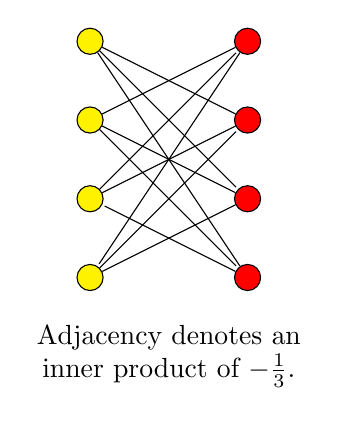
\begin{tikzpicture}[shorten >=1pt,auto,node distance=2cm,
		thin,main node/.style = {circle,draw}]
			\node[main node,fill=yellow] at (0,0) (1) {};
			\node[main node,fill=yellow] at (0,1) (2) {};
			\node[main node,fill=yellow] at (0,2) (3) {};
			\node[main node,fill=yellow] at (0,3) (4) {};
			\node[main node,fill=red] at (2,0) (5) {};
			\node[main node,fill=red] at (2,1) (6) {};
			\node[main node,fill=red] at (2,2) (7) {};
			\node[main node,fill=red] at (2,3) (8) {};
			\draw[-] (1) -- (6) -- (3) -- (8) -- (1);
			\draw[-] (2) -- (7) -- (4) -- (5) -- (2);
			\draw[-] (1) -- (7);
			\draw[-] (2) -- (8);
			\draw[-] (3) -- (5);
			\draw[-] (4) -- (6);
			\node[align=center] at (1,-1) () {Adjacency denotes an\\ inner product of $-\frac{1}{3}$.};		
		\end{tikzpicture}
	\end{column}
\end{columns}\end{frame}

\begin{frame}
\frametitle{Three fibers?}

		\[\begin{tikzpicture}[shorten >=1pt,auto,node distance=2cm,
		thin,main node/.style = {circle,draw}]
		\node[main node,fill=yellow] at (0,0) (y1) {};
		\node[main node,fill=yellow] at (-1,-1) (y2) {};
		\node[main node,fill=yellow] at (-2,-2) (y3) {};
		\node[main node,fill=yellow] at (-3,-3) (y4) {};
		\node[main node,fill=red] at (2,0) (r1) {};
		\node[main node,fill=red] at (3,-1) (r2) {};
		\node[main node,fill=red] at (4,-2) (r3) {};
		\node[main node,fill=red] at (5,-3) (r4) {};
		\node[main node,fill=black] at (-1.6,-5) (b1) {};
		\node[main node,fill=black] at (.2,-5) (b2) {};
		\node[main node,fill=black] at (1.8,-5) (b3) {};
		\node[main node,fill=black] at (3.6,-5) (b4) {};
		
		\only<1-3,6>{\draw[-] (y1)-- (r2);
		\draw[-] (y1)-- (r3);
		\draw[-] (y1)-- (r4);
		\draw[-] (y2)-- (r1);
		\draw[-] (y2)-- (r3);
		\draw[-] (y2)-- (r4);
		\draw[-] (y3)-- (r2);
		\draw[-] (y3)-- (r1);
		\draw[-] (y3)-- (r4);
		\draw[-] (y4)-- (r2);
		\draw[-] (y4)-- (r3);
		\draw[-] (y4)-- (r1);}
		\only<2-3,6>{
			\draw[-] (b1)-- (r2);
			\draw[-] (b1)-- (r3);
			\draw[-] (b1)-- (r4);
			\draw[-] (b2)-- (r1);
			\draw[-] (b2)-- (r3);
			\draw[-] (b2)-- (r4);
			\draw[-] (b3)-- (r2);
			\draw[-] (b3)-- (r1);
			\draw[-] (b3)-- (r4);
			\draw[-] (b4)-- (r2);
			\draw[-] (b4)-- (r3);
			\draw[-] (b4)-- (r1);}
		\only<3,6>{
			\draw[-] (y1)-- (b2);
			\draw[-] (y1)-- (b3);
			\draw[-] (y1)-- (b4);
			\draw[-] (y2)-- (b1);
			\draw[-] (y2)-- (b3);
			\draw[-] (y2)-- (b4);
			\draw[-] (y3)-- (b2);
			\draw[-] (y3)-- (b1);
			\draw[-] (y3)-- (b4);
			\draw[-] (y4)-- (b2);
			\draw[-] (y4)-- (b3);
			\draw[-] (y4)-- (b1);}
		\only<4-5>{\draw[-,very thin,gray] (y1)-- (r2);
			\draw[-,very thin,gray] (y1)-- (r3);
			\draw[-,very thin,gray] (y1)-- (r4);
			\draw[-,very thin,gray] (y2)-- (r1);
			\draw[-,very thin,gray] (y2)-- (r3);
			\draw[-,very thin,gray] (y2)-- (r4);
			\draw[-,very thin,gray] (y3)-- (r2);
			\draw[-,very thin,gray] (y3)-- (r1);
			\draw[-,very thin,gray] (y3)-- (r4);
			\draw[-,very thin,gray] (y4)-- (r2);
			\draw[-,very thin,gray] (y4)-- (r3);
			\draw[-,very thin,gray] (y4)-- (r1);
			\draw[-,very thin,gray] (b1)-- (r2);
			\draw[-,very thin,gray] (b1)-- (r3);
			\draw[-,very thin,gray] (b1)-- (r4);
			\draw[-,very thin,gray] (b2)-- (r1);
			\draw[-,very thin,gray] (b2)-- (r3);
			\draw[-,very thin,gray] (b2)-- (r4);
			\draw[-,very thin,gray] (b3)-- (r2);
			\draw[-,very thin,gray] (b3)-- (r1);
			\draw[-,very thin,gray] (b3)-- (r4);
			\draw[-,very thin,gray] (b4)-- (r2);
			\draw[-,very thin,gray] (b4)-- (r3);
			\draw[-,very thin,gray] (b4)-- (r1);
			\draw[-,very thin,gray] (y1)-- (b2);
			\draw[-,very thin,gray] (y1)-- (b3);
			\draw[-,very thin,gray] (y1)-- (b4);
			\draw[-,very thin,gray] (y2)-- (b1);
			\draw[-,very thin,gray] (y2)-- (b3);
			\draw[-,very thin,gray] (y2)-- (b4);
			\draw[-,very thin,gray] (y3)-- (b2);
			\draw[-,very thin,gray] (y3)-- (b1);
			\draw[-,very thin,gray] (y3)-- (b4);
			\draw[-,very thin,gray] (y4)-- (b2);
			\draw[-,very thin,gray] (y4)-- (b3);
			\draw[-,very thin,gray] (y4)-- (b1);}
		\only<4>{
			\draw[-,thick] (r1) -- (y2);
			\draw[-,red,thick] (r1)-- (b2);
			\draw[-,red,thick] (r1)-- (b3);
			\draw[-,red,thick] (r1)-- (b4);
			\draw[-,yellow,thick] (y2)-- (b1);
			\draw[-,yellow,thick] (y2)-- (b3);
			\draw[-,yellow,thick] (y2)-- (b4);	}
		\only<5>{
			\draw[dashed,thick] (r1) -- (y1);
			\draw[-,red,thick] (r1)-- (b2);
			\draw[-,red,thick] (r1)-- (b3);
			\draw[-,red,thick] (r1)-- (b4);
			\draw[-,yellow,thick] (y1)-- (b2);
			\draw[-,yellow,thick] (y1)-- (b3);
			\draw[-,yellow,thick] (y1)-- (b4);	}
		\end{tikzpicture}\]\pause\pause\pause\pause\pause
		\vspace{-1cm}
		\begin{center}
			Not representable as (distinct) simplices in $\mathbb{R}^3$
		\end{center}
\end{frame}

\begin{frame}
\frametitle{Def: Linked Systems of Symmetric Designs (Cameron)}
Let $\Gamma$ be a graph with vertex set $X$ and adjacency relation $\sim$. We say $\Gamma$ is a \textbf{linked system of symmetric $(v,k,\lambda)$ designs (LSSD) with $w$ fibers} if it is possible to partition $X$ into $w$ vertex subsets $X_1,\dots,X_w$ such that
\begin{itemize}
	\item no edge joins two vertices in the same fiber $X_i$;
	\item the subgraph induced between any $X_i$ and $X_j$ $(i\neq j)$ is the incidence graph of some symmetric $(v,k,\lambda)$ design (so $\vert X_i\vert = v$ for all $i$);
	\item for distinct $i,j,h$, if $a\in X_i$ and $b\in X_j$,
	\[\left\vert \Gamma(a)\cap\Gamma(b)\cap X_h\right\vert = \begin{cases}
	\mu \text{ if } a\sim b;\\
	\nu \text{ if } a\not\sim b.
	\end{cases} \]
\end{itemize}
\end{frame}



\begin{frame}
	\frametitle{LSSDs give cometric association schemes}
	\[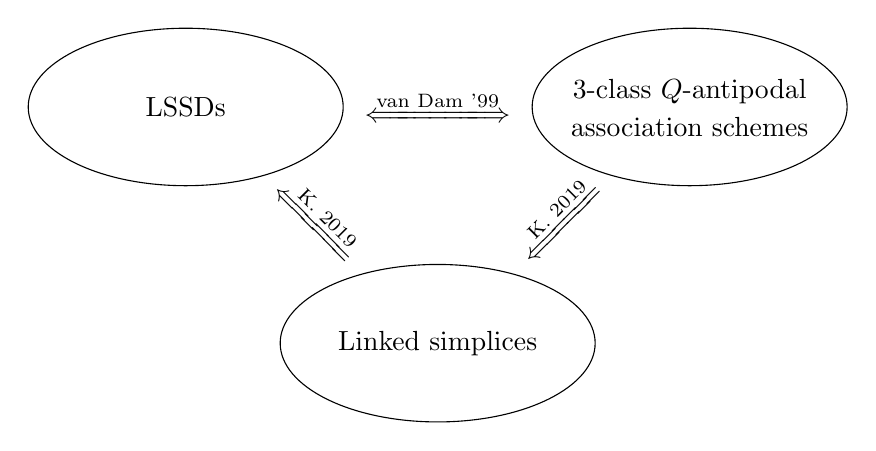
\begin{tikzpicture}
		\draw (-3.2,0) ellipse (2 and 1);
		\draw (3.2,0) ellipse (2 and 1);
		\node at (-3.2,0) (lssd) {LSSDs};
		\node at (3.2,.2) (assoc) {3-class $Q$-antipodal};
		\node at (3.2,-.25) (assoc2) {association schemes};
		\node at (0,0) (iff) {$\xLongleftrightarrow{\text{van Dam '99}}$};
		\onslide<2->{\draw (0,-3) ellipse (2 and 1);
		\node at (0,-3) (ls) {Linked simplices};}
		\onslide<3->{\node[rotate=45] at (1.6,-1.5) (if1) {$\xLongleftarrow{\text{K. 2019}}$};
		\node[rotate=-45] at (-1.6,-1.5) (if2) {$\xLongleftarrow{\text{K. 2019}}$};}
	\end{tikzpicture}\]
\end{frame}

\begin{frame}
\frametitle{Def: Linked Simplices}
Regular simplex:
\begin{itemize}
\item $v$ unit vectors spanning $\mathbb{R}^{v-1}$;
\item pairwise inner products of $-\frac{1}{v-1}$.
\end{itemize}
\vfill
Simplices $A$ and $B$ are ``linked" if there exists $-1\leq\gamma,\delta<1$ with:
\[\forall (a,b)\in A\times B: \left<a,b\right> \in\left\{\gamma,\delta\right\}\]
\vfill
Simplices $A_1,\dots,A_w$ are ``linked" if every pair is linked using the same constants.
\end{frame}

\begin{comment}

\begin{frame}
\frametitle{Linked Simplices vs. LSSDs}
\begin{thm}[K.]
	Let $\left\{a_i\right\}$ and $\left\{b_j\right\}$ be linked simplices in $\mathbb{R}^{v-1}$ with inner products $\gamma$ and $\delta$. For each $j$, let $B_j=\left\{a_i:\left<a_i,b_j\right>=\gamma\right\}$. Then $\left(\left\{a_i\right\},\left\{B_j\right\}\right)$ is a symmetric $2$-design.
\end{thm}
\begin{thm}[K.]
	Let $\left\{a_i\right\}$, $\left\{b_i\right\}$, and $\left\{c_i\right\}$ be three linked simplices in $\mathbb{R}^{v-1}$ with inner products $\gamma$ and $\delta$. For each $1\leq j,k\leq v$, let $B_j=\left\{a_i:\left<a_i,b_j\right>=\gamma\right\}$ and $C_k=\left\{a_i:\left<a_i,c_k\right>=\gamma\right\}$. Then there exists integers $\mu$ and $\nu$ such that
	\[\forall j,k: \left\vert B_j\cap C_k\right\vert = \begin{cases}
	\mu & \left<b_j,c_k\right> = \gamma\\
	\nu & \left<b_j,c_k\right> = \delta
	\end{cases}\]
\end{thm}
\end{frame}
\end{comment}

\begin{frame}
\frametitle{New LSSDs}
\begin{thm}[K.]
	Given a regular Hadamard matrix of order $s$ and an orthogonal array of size $s^2\times N$, there exists a $LSSD$ with $v=s^2$ and $w=N$.
\end{thm}\pause
\vfill
$H\in\left\{\pm1\right\}^{n\times n}$ is a Hadamard matrix of order $n$ if $HH^T = nI$.\pause
\vfill
An orthogonal array of size $s^2\times N$ is a set of $N$ columns with $s$ symbols where every ordered pair of symbols appears exactly once between columns.
\[O^T = \left[\begin{array}{cccccccccccccccc}
1 & 1 & 1 & 1 & 2 & 2 & 2 & 2 & 3 & 3 & 3 & 3 & 4 & 4 & 4 & 4\\
1 & 2 & 3 & 4 & 1 & 2 & 3 & 4 & 1 & 2 & 3 & 4 & 1 & 2 & 3 & 4\\
1 & 2 & 3 & 4 & 2 & 3 & 4 & 1 & 3 & 4 & 1 & 2 & 4 & 1 & 2 & 3\\
\end{array}\right]\]
\end{frame}

\begin{frame}
	\frametitle{Construction of an LSSD}\vspace{-.5cm}
	\[\left[\begin{array}{ccc}
	1 & 1 & 1\\
	1 & 2 & 2\\
	1 & 3 & 3\\
	1 & 4 & 4\\
	2 & 1 & 2\\
	2 & 2 & 3\\
	2 & 3 & 4\\
	2 & 4 & 1\\
	3 & 1 & 3\\
	3 & 2 & 4\\
	3 & 3 & 1\\
	3 & 4 & 2\\
	4 & 1 & 4\\
	4 & 2 & 1\\
	4 & 3 & 2\\
	4 & 4 & 3\\
	\end{array}\right]\qquad\longrightarrow\qquad \setlength{\arraycolsep}{0.8pt}{\left[\begin{array}{cccc|cccc|cccc}
		+&&& &+&&& &+&&&\\
		+&&& &&+&& &&+&&\\
		+&&& &&&+& &&&+&\\
		+&&& &&&&+ &&&&+\\
		&+&& &+&&& &&+&&\\
		&+&& &&+&& &&&+&\\
		&+&& &&&+& &&&&+\\
		&+&& &&&&+ &+&&&\\
		&&+& &+&&& &&&+&\\
		&&+& &&+&& &&&&+\\
		&&+& &&&+& &+&&&\\
		&&+& &&&&+ &&+&&\\
		&&&+ &+&&& &&&&+\\
		&&&+ &&+&& &+&&&\\
		&&&+ &&&+& &&+&&\\
		&&&+ &&&&+ &&&+&\\
		\end{array}\right]}\]
\end{frame}

\begin{frame}
\frametitle{Construction of an LSSD}
Using $H = \left[\begin{array}{rrrr}
- & + & + & +\\
+ & - & + & +\\
+ & + & - & +\\
+ & + & + & -\\
\end{array}\right]$,
\[\begin{aligned}\hspace{-2mm}
\setlength{\arraycolsep}{0.8pt}{\fontsize{5}{6}\selectfont\left[\begin{array}{cccc}
	+&&&\\
	+&&&\\
	+&&&\\
	+&&&\\
	&+&&\\
	&+&&\\
	&+&&\\
	&+&&\\
	&&+&\\
	&&+&\\
	&&+&\\
	&&+&\\
	&&&+\\
	&&&+\\
	&&&+\\
	&&&+\\
	\end{array}\right]}\rightarrow\setlength{\arraycolsep}{0.4pt}{\fontsize{5}{6}\selectfont\left[\begin{array}{rrrr|rrrr|rrrr|rrrr}
	- & + & + & +&&&&&&&&&&&&\\
	+ & - & + & +&&&&&&&&&&&&\\
	+ & + & - & +&&&&&&&&&&&&\\
	+ & + & + & -&&&&&&&&&&&&\\
	&&&&- & + & + & +&&&&&&&&\\
	&&&&+ & - & + & +&&&&&&&&\\
	&&&&+ & + & - & +&&&&&&&&\\
	&&&&+ & + & + & -&&&&&&&&\\
	&&&&&&&&- & + & + & +&&&&\\
	&&&&&&&&+ & - & + & +&&&&\\
	&&&&&&&&+ & + & - & +&&&&\\
	&&&&&&&&+ & + & + & -&&&&\\
	&&&&&&&&&&&&- & + & + & +\\
	&&&&&&&&&&&&+ & - & + & +\\
	&&&&&&&&&&&&+ & + & - & +\\
	&&&&&&&&&&&&+ & + & + & -\\
	\end{array}\right]}
\end{aligned}\]
\end{frame}

\begin{frame}
	\frametitle{Construction of an LSSD}
	Similarly we get the two additional arrays
	\[\begin{aligned}\setlength{\arraycolsep}{0.4pt}{\fontsize{5}{6}\selectfont\left[\begin{array}{rrrr|rrrr|rrrr|rrrr}
			- & + & + & +&&&&&&&&&&&&\\
			&&&&- & + & + & +&&&&&&&&\\
			&&&&&&&&- & + & + & +&&&&\\
			&&&&&&&&&&&&- & + & + & +\\
			+ & - & + & +&&&&&&&&&&&&\\
			&&&&+ & - & + & +&&&&&&&&\\
			&&&&&&&&+ & - & + & +&&&&\\
			&&&&&&&&&&&&+ & - & + & +\\
			+ & + & - & +&&&&&&&&&&&&\\
			&&&&+ & + & - & +&&&&&&&&\\
			&&&&&&&&+ & + & - & +&&&&\\
			&&&&&&&&&&&&+ & + & - & +\\
			+ & + & + & -&&&&&&&&&&&&\\
			&&&&+ & + & + & -&&&&&&&&\\
			&&&&&&&&+ & + & + & -&&&&\\
			&&&&&&&&&&&&+ & + & + & -\\
		\end{array}\right]},\quad&\setlength{\arraycolsep}{0.4pt}{\fontsize{5}{6}\selectfont\left[\begin{array}{rrrr|rrrr|rrrr|rrrr}
			- & + & + & +&&&&&&&&&&&&\\
			&&&&- & + & + & +&&&&&&&&\\
			&&&&&&&&- & + & + & +&&&&\\
			&&&&&&&&&&&&- & + & + & +\\
			&&&&+ & - & + & +&&&&&&&&\\
			&&&&&&&&+ & - & + & +&&&&\\
			&&&&&&&&&&&&+ & - & + & +\\
			+ & - & + & +&&&&&&&&&&&&\\
			&&&&&&&&+ & + & - & +&&&&\\
			&&&&&&&&&&&&+ & + & - & +\\
			+ & + & - & +&&&&&&&&&&&&\\
			&&&&+ & + & - & +&&&&&&&&\\
			&&&&&&&&&&&&+ & + & + & -\\
			+ & + & + & -&&&&&&&&&&&&\\
			&&&&+ & + & + & -&&&&&&&&\\
			&&&&&&&&+ & + & + & -&&&&\\
		\end{array}\right]}.
\end{aligned}\]
\end{frame}

\begin{frame}\frametitle{Construction of an LSSD}
Taking inner products, we get the Hadamard matrices
\[\begin{aligned}
H_{1,2}=\setlength{\arraycolsep}{.8pt}{\fontsize{5}{6}\selectfont\left[\begin{array}{rrrrrrrrrrrrrrrr}
	+&-&-&-&-&+&+&+&-&+&+&+&-&+&+&+\\
	-&+&+&+&+&-&-&-&-&+&+&+&-&+&+&+\\
	-&+&+&+&-&+&+&+&+&-&-&-&-&+&+&+\\
	-&+&+&+&-&+&+&+&-&+&+&+&+&-&-&-\\
	-&+&-&-&+&-&+&+&+&-&+&+&+&-&+&+\\
	+&-&+&+&-&+&-&-&+&-&+&+&+&-&+&+\\
	+&-&+&+&+&-&+&+&-&+&-&-&+&-&+&+\\
	+&-&+&+&+&-&+&+&+&-&+&+&-&+&-&-\\
	-&-&+&-&+&+&-&+&+&+&-&+&+&+&-&+\\
	+&+&-&+&-&-&+&-&+&+&-&+&+&+&-&+\\
	+&+&-&+&+&+&-&+&-&-&+&-&+&+&-&+\\
	+&+&-&+&+&+&-&+&+&+&-&+&-&-&+&-\\
	-&-&-&+&+&+&+&-&+&+&+&-&+&+&+&-\\
	+&+&+&-&-&-&-&+&+&+&+&-&+&+&+&-\\
	+&+&+&-&+&+&+&-&-&-&-&+&+&+&+&-\\
	+&+&+&-&+&+&+&-&+&+&+&-&-&-&-&+\\
	\end{array}\right]},\quad
&H_{1,3}=\setlength{\arraycolsep}{.8pt}{\fontsize{5}{6}\selectfont\left[\begin{array}{rrrrrrrrrrrrrrrr}
	+&-&-&-&-&+&+&+&-&+&+&+&-&+&+&+\\
	-&+&+&+&+&-&-&-&-&+&+&+&-&+&+&+\\
	-&+&+&+&-&+&+&+&+&-&-&-&-&+&+&+\\
	-&+&+&+&-&+&+&+&-&+&+&+&+&-&-&-\\
	+&-&+&+&-&+&-&-&+&-&+&+&+&-&+&+\\
	+&-&+&+&+&-&+&+&-&+&-&-&+&-&+&+\\
	+&-&+&+&+&-&+&+&+&-&+&+&-&+&-&-\\
	-&+&-&-&+&-&+&+&+&-&+&+&+&-&+&+\\
	+&+&-&+&+&+&-&+&-&-&+&-&+&+&-&+\\
	+&+&-&+&+&+&-&+&+&+&-&+&-&-&+&-\\
	-&-&+&-&+&+&-&+&+&+&-&+&+&+&-&+\\
	+&+&-&+&-&-&+&-&+&+&-&+&+&+&-&+\\
	+&+&+&-&+&+&+&-&+&+&+&-&-&-&-&+\\
	-&-&-&+&+&+&+&-&+&+&+&-&+&+&+&-\\
	+&+&+&-&-&-&-&+&+&+&+&-&+&+&+&-\\
	+&+&+&-&+&+&+&-&-&-&-&+&+&+&+&-\\
	\end{array}\right]},\end{aligned}\]\[H_{2,3}=\setlength{\arraycolsep}{.8pt}{\fontsize{5}{6}\selectfont\left[\begin{array}{rrrrrrrrrrrrrrrr}
	+&-&-&-&+&-&+&+&+&+&-&+&+&+&+&-\\
	-&+&+&+&-&+&-&-&+&+&-&+&+&+&+&-\\
	-&+&+&+&+&-&+&+&-&-&+&-&+&+&+&-\\
	-&+&+&+&+&-&+&+&+&+&-&+&-&-&-&+\\
	+&+&+&-&+&-&-&-&+&-&+&+&+&+&-&+\\
	+&+&+&-&-&+&+&+&-&+&-&-&+&+&-&+\\
	+&+&+&-&-&+&+&+&+&-&+&+&-&-&+&-\\
	-&-&-&+&-&+&+&+&+&-&+&+&+&+&-&+\\
	+&+&-&+&+&+&+&-&+&-&-&-&+&-&+&+\\
	+&+&-&+&+&+&+&-&-&+&+&+&-&+&-&-\\
	-&-&+&-&+&+&+&-&-&+&+&+&+&-&+&+\\
	+&+&-&+&-&-&-&+&-&+&+&+&+&-&+&+\\
	+&-&+&+&+&+&-&+&+&+&+&-&+&-&-&-\\
	-&+&-&-&+&+&-&+&+&+&+&-&-&+&+&+\\
	+&-&+&+&-&-&+&-&+&+&+&-&-&+&+&+\\
	+&-&+&+&+&+&-&+&-&-&-&+&-&+&+&+\\
	\end{array}\right]}.
\]
\end{frame}

\begin{frame}
\frametitle{Construction of an LSSD}
Then
\[M = \frac{1}{12}\left[\begin{array}{ccc}
4I & H_{12}& H_{13}\\
H_{12}^T & 4I & H_{23}\\
H_{13}^T& H_{23}^T & 4I
\end{array}\right]\]
is a rank $16$ idempotent and
\[\frac{48}{15}\left(M-\frac{1}{48}J\right)\]
is the Gram matrix of a set of linked simplices.
\end{frame}

\begin{comment}
\begin{frame}
\begin{cor}[K.]
	For sufficiently large $s$, there exists a $LSSD(s^2,k,\lambda;w)$ with $w\geq s^\frac{1}{14.8}$ if there exists a regular Hadamard matrix of order $s$.
\end{cor}
\begin{cor}[K.]
	For any $n\geq 1$ and $w>2$, there exists an odd $t$ for which a $LSSD(16^{n}t,k,\lambda;w)$ exists.
\end{cor}
\end{frame}
\end{comment}

%\begin{frame}
%\frametitle{Table of new LSSDs}
%Given a regular Hadamard matrix of order $4t^2$, there exists a $LSSD(16t^4,k,\lambda;w(t))$.\vfill
%\scalebox{.7}{\begin{tabular}{c|*{17}{c}}
%		$t$ & 1 & 2 & 3 & 4 & 5 & 6 & 7 & 8 & 9 & 10& 11 & 12 & 13 & 14 & 15 & 16 & 17 \\\hline
%		$w(t)$&5&17&9&65&10&12&8&257&10&17&17&10&10&10&29&1025&10\\\\
%		$t$ & 18 & 19 & 20& 21 & 22 & 23 & 24 & 25 & 26 & 27 & 28 & 29 & 30& 31 & 32 & 33 \\\hline
%		$w(t)$&26&11&26&11&17&11&32&10&17&10&50&30&30&12&4097&32\\\\
%		$t$ & 34 & 35 & 36 & 37 & 38 & 39 & 40 & 41 & 42 & 43 & 44 & 45 & 46 & 47 & 48 & 49 &\\\hline
%		$w(t)$&18&32&65&32&18&32&26&13&20&32&65&17&32&32&30&17
%\end{tabular}}\vfill
%\end{frame}

\section{Other questions/topics}

\begin{frame}
\frametitle{Equiangular lines related to association schemes}
\begin{lemma}[K.]
	Let $\mathbb{A}$ be a Bose-Mesner algebra with second eigenmatrix $Q$ and multiplicities $m_0,\dots,m_d$. Define $Q^\prime$ to be the submatrix of $Q$ given by deleting row $0$. If there exists a non-negative vector $x$ so that $Q^\prime x\in\left\{-1,1\right\}^d$, then $\mathbb{A}$ contains the Gram matrix of $\vert X\vert$ equiangular lines in dimension $n=\sum_{x_j\neq 0} m_j$ with angle $\alpha =\left(\sum x_jm_j\right)^{-1}$.
\end{lemma}
\end{frame}
\begin{frame}[allowframebreaks]
\frametitle{Effect of Gegenbaur polynomails}
\begin{theorem}[K.,Martin]
	Suppose we have a feasible parameter set for an association scheme with first and second eigenmatrices $P$ and $Q$. Fix $0\leq i\leq d$ and set $m_i:=Q_{0i}$. For $\ell>0$ define $\mu_\ell = \frac{\ell-1}{\ell+m_i-3}$ and $\lambda_j = \nicefrac{Q_{ji}}{Q_{0i}}$. Let $\gamma_{\ell,j}$ equal $\lambda_j^2$ if $(1+\mu_\ell)^2\lambda_j^2\geq 4\mu_\ell$ and $\mu_\ell$ otherwise. Then all entries of $Q_{\ell^*}^{m_i}\left(\frac{1}{m_i}L_i^*\right)$ are non-negative whenever
	\[\sum_{j=1}^d \left(\prod_{\ell=2}^{\ell^*+1}\gamma_{x,j}\right)P_{0j}\left(1+\lambda_j^2\right)\leq\frac{1}{\vert X\vert}.\]
\end{theorem}

\begin{theorem}[K.,Martin]
	Suppose we have a feasible parameter set for a cometric association scheme with Krein array $\iota^*(X,\mathcal{R}) = \left\{m,b^*_1,\dots,b^*_{d-1};1,c_2^*\dots,c^*_{d}\right\}$ where $m>2$. Define $b_{j-1}^* = c_j^*=a_j^*=0$ for $j>d$. Then the scheme is realizable only if
	\begin{itemize}
		\item $\left(a_1^*\right)^2 + b_1^*c_2^* \geq\frac{2m(m-1)}{m+2},$
		\item $\left(a_1^*\right)^2+2a_1^*a_2^*+c_2^*q^2_{22}\geq \frac{4m(m-2)}{m+4},$
		\item $\frac{6m(m-1)(m-4)}{(m+4)(m+6)}+\frac{\left(3a_1^*\left(a_1^*+a_2^*\right)+c_2^*q_{22}^2\right)b_1^*c_2^*+\left(a_1^*\right)^4}{m}\geq \frac{(7m-18)\left(\left(a_1^*\right)^2+b_1^*c_2^*\right)}{m+6},$
		\item $\sum_{i=1}^3\left(b_i^*c_{i+1}^* + a_i^*\sum_{j=i}^3 a_j^*\right)\leq \frac{3(3m-2)}{m+6}.$
		\item $\frac{16m(m-1)}{(m+4)(m+8)} + \frac{\left(a_1^*\right)^4 + \left(3a_1^*\left(a_1^*+a_2^*\right)+c_2^*q_{22}^2\right)b_1^*c_2^*}{(m-2)m}\geq \frac{12\left(\left(a_1^*\right)^2+b_1^*c_2^*\right)}{m+8},$
	\end{itemize}
	Additionally, if $a_1^*>0$, then
	\begin{itemize}
		\item $\left(a_1^*\right)^2 + b_1^*c_2^*\left(2 + \frac{a_2^*}{a_1^*}\right)\geq \frac{4m(2m-3)}{m+6},$
		\item $\left(a_1^*\right)^2+2a_1^*a_2^*-\left(a_2^*\right)^2+2c_2^*q_{22}^2+\frac{b_2^*c_3^*\left(a_3^*-a_1^*\right)-ma_2^*}{a_1^*+a_2^*}\geq\frac{6m(m-4)}{m+6}.$
	\end{itemize}
\end{theorem}
\end{frame}
\begin{frame}[allowframebreaks]
\frametitle{LSSDs coming from unbiased Hadamard matrices}
\begin{theorem}[K.]
	A $LSSD(v,k,\lambda;w)$ is equivalent to a set of $w$ linked simplices in $\mathbb{R}^{v-1}$ with angles given by $(4.8)$.
\end{theorem}

\begin{theorem}[K.]
	\label{equiv}
	An optimistic $LSSD(v,k,\lambda;w)$ with $\vert v-2k\vert = 2\sqrt{k-\lambda}$ exists if and only if there exists a set of $w-1$ regular unbiased Hadamard matrices, $H_i$, with order $v$ and $H_iJ = 2\sqrt{k-\lambda}J$.
\end{theorem}

\begin{theorem}[K.]
	\label{asymptotics}
	For sufficiently large $n$, if there exists a regular Hadamard matrix of order $n$, then there exists a $LSSD(n^2,k,\lambda; w)$ with $w \geq n^\frac{1}{14.8}$.
\end{theorem}

\begin{theorem}[K.]
	For any $n\geq 1$ and $w>2$, there exists an $LSSD(16^nt,k,\lambda;w)$ for some odd $t$.
\end{theorem}

\begin{theorem}[K.]
	There exists an $LSSD(v,k,\lambda;w)$ with $v=36^{2n}$ and $w = 4^n+1$ for all $n\geq 1$.
\end{theorem}
\end{frame}


\begin{frame}
\frametitle{Orthogonal projective doubles}

\[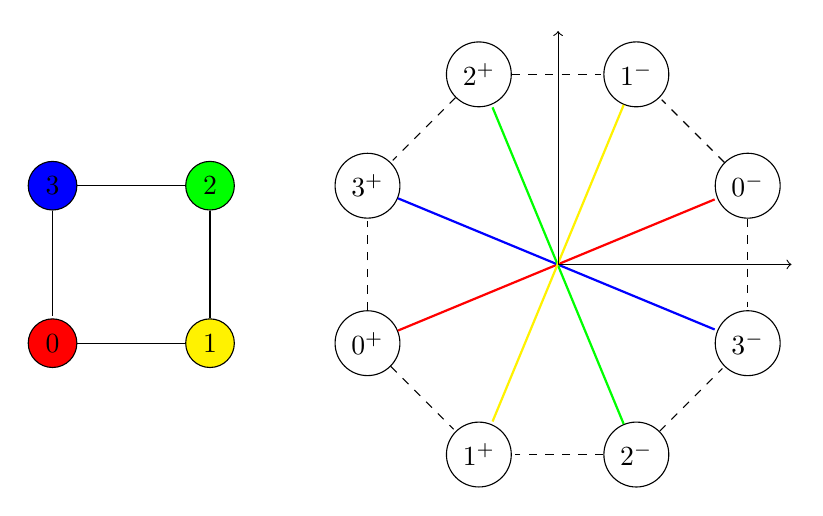
\begin{tikzpicture}[shorten >=1pt,auto,node distance=2cm,
thin,main node/.style = {circle,draw}]
	\node[main node,fill=red] at (0,0) (0) {0};
	\node[main node,fill=yellow] at (2,0) (1) {1};
	\node[main node,fill=green] at (2,2) (2) {2};
	\node[main node,fill=blue] at (0,2) (3) {3};
	
	\path[draw,-] (0) -- (1) -- (2) -- (3) -- (0);
	\pause
	\node[main node,fill=white] [right of =1 ](11) {$0^+$};
	\node[main node,fill=white] [below right of = 11](22) {$1^+$};
	\node[main node,fill=white] [above of = 11](33) {$3^+$};
	\node[main node,fill=white] [above right of =33](44) {$2^+$};

	\node[main node,fill=white] [right of =22](5) {$2^-$};
	\node[main node,fill=white] [above right of = 5](6) {$3^-$};
	\node[main node,fill=white] [right of = 44](7) {$1^-$};
	\node[main node,fill=white] [below right of =7](8) {$0^-$};
	
	
	\path[-,dashed]
	(11) edge node {} (22)
	edge node {} (33)
	(44) edge node {} (33)
	edge node {} (7)
	(5) edge node {} (6)
	edge node {} (22)
	(8) edge node {} (7)
	edge node {} (6);
	\draw[-, red,thick] (11) -- (8);
	\draw[-, blue,thick] (33) -- (6);
	\draw[-, green,thick] (5) -- (44);
	\draw[-, yellow,thick] (7) -- (22);
	\draw[->] (6.42,1) -> (6.42,4);
	\draw[->] (6.42,1) -> (9.42,1);
	
	
\end{tikzpicture}\]
\end{frame}

\begin{frame}[allowframebreaks]
\frametitle{Orthogonal projective doubles}

\begin{proposition}[K.,Martin]
	An $OPD_m(\Gamma;\beta)$ for simple graph $\Gamma$ induces an association scheme only if $\Gamma$ is strongly regular.
\end{proposition}

\begin{corollary}[K.,Martin]
	Let $\Gamma$ be a connected strongly regular graph with $v$ vertices and eigenvalues $k>r>s$ which contains a Delsarte coclique $C$ of size $m$. Then an $OPD_{m}(\Gamma;\beta)$ exists only if $\beta=\frac{1}{\sqrt{-s}}$. Further, either $\Gamma$ is complete bipartite or $\beta^{-1}\in \mathbb{Z}$.
\end{corollary}

\begin{corollary}[K.,Martin]
	Let $\Gamma$ be a connected strongly regular graph with $v$ vertices and eigenvalues $k>r>s$. An $OPD_{m}(\Gamma;\beta)$ with $m<v$ induces an association scheme if and only if $m = v\left(1+k\beta^2\right)^{-1}$.
\end{corollary}

\begin{theorem}[K.,Martin]
	Suppose we have a feasible parameter set for a $4$-class association scheme which is $Q$-bipartite but not $Q$-antipodal. Let $k=P_{01}$, $r=P_{21}$, and $s=P_{41}$ where $P$ is the first eigenmatrix using the natural ordering. Then the scheme is realizable only if $s=-n^2$ for some integer $n>1$ and
	\[15n^4(2n^2-3)r^2 + (n^6-45kn^2+76k)n^2r+k(16k+n^6)(n^2-2)\geq 0.\]
\end{theorem}
\end{frame}
\begin{frame}[allowframebreaks]
\frametitle{Connectivity of association schemes}
\begin{theorem}[K.,Martin] \label{Tmain}
	Let $(X,\mathcal{R})$ be a symmetric association scheme. Assume the graph $\Gamma=\Gamma(X,R_i)$ is connected 
	and not complete multipartite. Let
	$H=H_i$ be the corresponding unweighted distribution diagram on $\{0,1,\ldots, d\}$. The following are equivalent:
	%%%%%%%%%%%%  JUNE 16  : check if vertex set is smaller than {0,1,..,d} when not symmetric
	\begin{itemize}
		\item[(1)] there exists $a\in X$ for which the subgraph $\Gamma \setminus a^\bot$ is connected;
		\item[(2)] for all $a\in X$, the subgraph $\Gamma \setminus a^\bot$ is connected;
		\item[(3)]  the subgraph $H \setminus \{0,i\}$ is connected;
		\item[(4)] $\Gamma$ contains no twins.
	\end{itemize} 
\end{theorem}

\begin{corollary}[K.,Martin]  \label{C2}
	Let $(X,\mathcal{R})$ be a commutative association scheme. Assume the undirected graph 
	$\Gamma=\Gamma(X,R_i  \cup R_{i'})$ is connected and $a\in X$. Then $\Gamma \setminus 
	\Gamma(a)$ contains at most one non-singleton component.
\end{corollary}


\begin{corollary}[K.,Martin] \label{C1}
	Let $(X,\mathcal{R})$ be a commutative association scheme.  Assume the undirected graph 
	$\Gamma=\Gamma(X,R_i  \cup R_{i'})$ is connected and $a\in X$.  Then, for any  $T \subseteq a^\bot$ with $\Gamma(a) \not\subseteq T$, the graph  $\Gamma \setminus T$ is connected.
\end{corollary}

\begin{corollary}[K.,Martin] \label{C3}
	Let $(X,\mathcal{R})$ be a commutative association scheme. Assume the undirected graph 
	$\Gamma=\Gamma(X,R_i  \cup R_{i'})$ is connected and $C\subseteq  X$ is the vertex set of a clique in $\Gamma$. Then $\Gamma \setminus C$ is connected.
\end{corollary}


\begin{theorem}[K.,Martin]
	\label{Tcutsize2}
	Let $(X,\mathcal{R})$ be a symmetric association scheme and let $\Gamma=\Gamma(X,R_1)$  be the graph 
	associated to a connected basis relation. If $\Gamma$ admits a  disconnecting set of size two, 
	then $\Gamma$ is isomorphic to a polygon.
\end{theorem}

\begin{theorem}[K.,Martin]
	\label{Tcutsize3}
	Let $(X,\mathcal{R})$ be a symmetric association scheme and let $\Gamma=\Gamma(X,R_1)$  be the graph 
	associated to a connected basis relation. If $\Gamma$ has diameter two, then either
	$\Gamma$ has vertex connectivity at least four or
	$\Gamma$ is isomorphic to one of the following graphs: the  4-cycle, the 5-cycle, $K_{3,3}$, 
	the Petersen graph.
\end{theorem}

\begin{lemma}[K.,Martin]
	\label{Lspec-cut}
	Let $(X,\mathcal{R})$ be a symmetric association scheme and let $\Gamma=\Gamma(X,R_1)$ be the graph associated to a con\-nec\-ted basis relation.
	Assume that $\Gamma$ contains no induced subgraph isomorphic to $K_{2,1,1}$. 
	If  $T\subseteq X$ is a disconnecting set for $\Gamma$, then $|T|> p_{11}^1$.
\end{lemma}

\end{frame}

\begin{frame}[noframenumbering]
\frametitle{Acknowledgements}
Adviser:
\begin{itemize}
	\item Dr. William Martin, WPI
\end{itemize}
Dissertation Committee:
\begin{itemize}
	\item Dr. Peter J. Cameron, Queen Mary, University of London
	\item Dr. Padraig \'{O} Cath\'{a}in, WPI
	\item Dr. Peter R. Christopher, WPI
	\item Dr. William M. Kantor, University of Oregon
	\item Dr. G\'{a}bor N. S\'{a}rk\"{o}zy, WPI
\end{itemize}
\end{frame}


\end{document}
